\documentclass[]{article}
\usepackage{amsfonts, amssymb, amsmath}
\usepackage{float}
\usepackage{graphicx}
\usepackage{pgfplots}

\title{Gate 64.2022}
\author{Umair Parwez \\ EE22BTECH11009}
\date{}
\begin{document}
\maketitle
\providecommand{\pr}[1]{\ensuremath{\Pr\left(#1\right)}}
\providecommand{\prt}[2]{\ensuremath{p_{#1}^{\left(#2\right)} }}        % own macro for this question
\providecommand{\qfunc}[1]{\ensuremath{Q\left(#1\right)}}
\providecommand{\sbrak}[1]{\ensuremath{{}\left[#1\right]}}
\providecommand{\lsbrak}[1]{\ensuremath{{}\left[#1\right.}}
\providecommand{\rsbrak}[1]{\ensuremath{{}\left.#1\right]}}
\providecommand{\brak}[1]{\ensuremath{\left(#1\right)}}
\providecommand{\lbrak}[1]{\ensuremath{\left(#1\right.}}
\providecommand{\rbrak}[1]{\ensuremath{\left.#1\right)}}
\providecommand{\cbrak}[1]{\ensuremath{\left\{#1\right\}}}
\providecommand{\lcbrak}[1]{\ensuremath{\left\{#1\right.}}
\providecommand{\rcbrak}[1]{\ensuremath{\left.#1\right\}}}
\newcommand{\sgn}{\mathop{\mathrm{sgn}}}
\providecommand{\abs}[1]{\left\vert#1\right\vert}
\providecommand{\res}[1]{\Res\displaylimits_{#1}} 
\providecommand{\norm}[1]{\left\lVert#1\right\rVert}
%\providecommand{\norm}[1]{\lVert#1\rVert}
\providecommand{\mtx}[1]{\mathbf{#1}}
\providecommand{\mean}[1]{E\left[ #1 \right]}
\providecommand{\cond}[2]{#1\middle|#2}
\providecommand{\fourier}{\overset{\mathcal{F}}{ \rightleftharpoons}}
\newenvironment{amatrix}[1]{%
  \left(\begin{array}{@{}*{#1}{c}|c@{}}
}{%
  \end{array}\right)
}
%\providecommand{\hilbert}{\overset{\mathcal{H}}{ \rightleftharpoons}}
%\providecommand{\system}{\overset{\mathcal{H}}{ \longleftrightarrow}}
	%\newcommand{\solution}[2]{\textbf{Solution:}{#1}}
\newcommand{\solution}{\noindent \textbf{Solution: }}
\newcommand{\cosec}{\,\text{cosec}\,}
\providecommand{\dec}[2]{\ensuremath{\overset{#1}{\underset{#2}{\gtrless}}}}
\newcommand{\myvec}[1]{\ensuremath{\begin{pmatrix}#1\end{pmatrix}}}
\newcommand{\mydet}[1]{\ensuremath{\begin{vmatrix}#1\end{vmatrix}}}
\newcommand{\myaugvec}[2]{\ensuremath{\begin{amatrix}{#1}#2\end{amatrix}}}
\providecommand{\rank}{\text{rank}}
\providecommand{\pr}[1]{\ensuremath{\Pr\left(#1\right)}}
\providecommand{\qfunc}[1]{\ensuremath{Q\left(#1\right)}}
	\newcommand*{\permcomb}[4][0mu]{{{}^{#3}\mkern#1#2_{#4}}}
\newcommand*{\perm}[1][-3mu]{\permcomb[#1]{P}}
\newcommand*{\comb}[1][-1mu]{\permcomb[#1]{C}}
\providecommand{\qfunc}[1]{\ensuremath{Q\left(#1\right)}}
\providecommand{\gauss}[2]{\mathcal{N}\ensuremath{\left(#1,#2\right)}}
\providecommand{\diff}[2]{\ensuremath{\frac{d{#1}}{d{#2}}}}
\providecommand{\myceil}[1]{\left \lceil #1 \right \rceil }
\newcommand\figref{Fig.~\ref}
\newcommand\tabref{Table~\ref}
\newcommand{\sinc}{\,\text{sinc}\,}
\newcommand{\rect}{\,\text{rect}\,}
%%
%	%\newcommand{\solution}[2]{\textbf{Solution:}{#1}}
%\newcommand{\solution}{\noindent \textbf{Solution: }}
%\newcommand{\cosec}{\,\text{cosec}\,}
%\numberwithin{equation}{section}
%\numberwithin{equation}{subsection}
%\numberwithin{problem}{section}
%\numberwithin{definition}{section}
%\makeatletter
%\@addtoreset{figure}{problem}
%\makeatother

%\let\StandardTheFigure\thefigure
\let\vec\mathbf

Consider a real valued source whose samples are independent and identically
distributed random variables with the probability density function, $P_X(x)$, as shown in
the figure.

\begin{center}
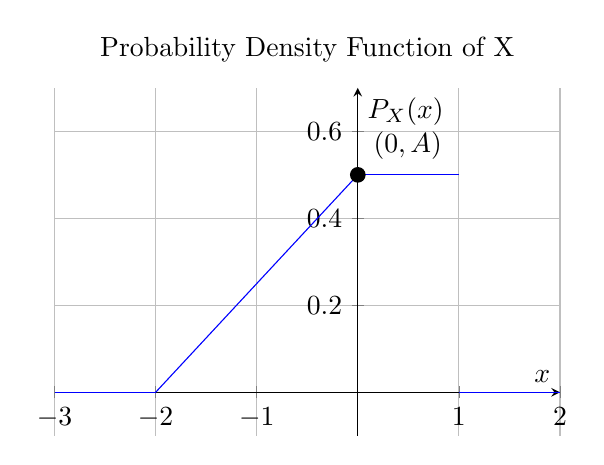
\begin{tikzpicture}
    \begin{axis}[
        xlabel=$x$,
        ylabel=$P_X(x)$,
        title=Probability Density Function of X,
        grid=both,
        axis lines=middle,
        xmax=2,
        xmin=-3,
        ymax=0.7,
        ymin=-0.1,
        width=8cm,
        height=6cm,
        legend style={at={(0.05,0.95)},anchor=north west}
    ]
    \addplot[blue,mark=none,domain=-2:0,samples=100] {0.25*x + 0.5};
    \addplot[blue,mark=none,domain=0:1,samples=100] {0.5};
    \addplot[blue,mark=none,domain=-3:-2,samples=100] {0};
    \addplot[blue,mark=none,domain=1:2,samples=100] {0};
    \node[label={45:{$(0,A)$}},circle,fill,inner sep=2pt] at (axis cs:0,0.5) {};
    \end{axis}
\end{tikzpicture}
\end{center}

Consider a 1 bit quantizer that maps positive samples to value $\alpha$ and others to value
$\beta$. If $\alpha ^*$ and $\beta ^*$ are the respective choices for $\alpha$ and $\beta$ that minimize the mean square
quantization error, then find ($\alpha ^* - \beta ^*$)

\solution
First we must find value of A. Area under the PDF graph should be equal to 1. Thus, we can say,
\begin{align}
    \brak{\frac{1}{2}\cdot A\cdot 2} + (1\cdot A) = 1 \\
    A = 0.5
\end{align}

Using the value of A, we can write $P_X(x)$ as a piecwise function given by,
\begin{align}
    p_X(x) = 
    \begin{cases}
        0.25x + 0.5 & -2\leq x\leq 0 \\
        0.5 & 0\leq x \leq1
    \end{cases}
\end{align}

Now, if $X_q$ be the output of the quantizer, then,
\begin{align}
    X_q = 
    \begin{cases}
        \alpha & 0\leq x \leq1 \\
        \beta & -2\leq x\leq 0
    \end{cases}
\end{align}

Now, the quantization error, $Q_e$, is given by,
\begin{align}
    Q_e = X-X_q
\end{align}

Mean square quantization error, 
\begin{align}
    MSQE &= E(Q_e^2) \\
    &= E((X-X_q)^2) \\
    &= \int_{-\infty}^{\infty}(x-X_q)^2\cdot P_X(x)\cdot dx \\
    &= \int_{-2}^{0}(x-\beta)^2\cdot P_X(x)\cdot dx + \int_{0}^{1}(x-\alpha)^2\cdot P_X(x)\cdot dx \\
    &= \int_{-2}^{0}(x^2+\beta ^2-2x\beta)\cdot (0.25x+0.5)\cdot dx \\ &\qquad + \int_{0}^{1}(x-\alpha)^2\cdot 0.5\cdot dx \\
    &= \frac{\beta ^2}{2} + \frac{2\beta}{3} -\frac{1}{3} + \frac{1}{6}[(1-\alpha)^3+\alpha ^3] \\
    &= (\frac{\beta ^2}{2} + \frac{2\beta}{3}) + \frac{1}{2}(\alpha ^2 - \alpha) - \frac{1}{6} \\
    &= \frac{\alpha ^2}{2} + \frac{\beta ^2}{2} - \frac{\alpha}{2} + \frac{2\beta}{3} - \frac{1}{6} 
\end{align}

Now, we can write MSQE as,
\begin{align}
    f(\mathbf{v}) = \mathbf{v}^\intercal \mathbf{A} \mathbf{v} + 2 \mathbf{B} \mathbf{v} - \frac{1}{6}
\end{align}

Where, 
\begin{align}
    \mathbf{v} = 
    \begin{bmatrix}
        \alpha \\
        \beta
    \end{bmatrix};
    A =
    \begin{bmatrix}
        \frac{1}{2} & 0 \\
        0 & \frac{1}{2}
    \end{bmatrix}; 
    B = 
    \begin{bmatrix}
        \frac{-1}{4} & \frac{1}{3}
    \end{bmatrix}
\end{align}

Now, to minimize $MSQE$,
\begin{align}
    \frac{d}{d \mathbf{v}} f(\mathbf{v}) = 
    \begin{bmatrix}
        0\\
        0
    \end{bmatrix} \\
    (A+A^\intercal)\mathbf{v} + 2B^\intercal = 
    \begin{bmatrix}
        0\\
        0
    \end{bmatrix} \\
\end{align}

Since A is a symmetric matrix, $A^\intercal = A$. Therefore, 
\begin{align}
    2A \mathbf{v} &= -2B^\intercal \\
    \mathbf{v} &= -A^{-1}B^\intercal \\
    &= -
    \begin{bmatrix}
        2 & 0\\
        0 & 2
    \end{bmatrix}
    \begin{bmatrix}
        \frac{-1}{4} \\
        \frac{1}{3}
    \end{bmatrix} \\
    &= 
    \begin{bmatrix}
        \frac{1}{2}\\
        \frac{-2}{3} 
    \end{bmatrix}
\end{align}

Now, to find $(\alpha ^* - \beta ^*)$, 
\begin{align}
    (\alpha ^* - \beta ^*) &= 
    \begin{bmatrix}
        1 & -1
    \end{bmatrix} \mathbf{v} \\
    &= 
    \begin{bmatrix}
        1 & -1
    \end{bmatrix}
    \begin{bmatrix}
        \frac{1}{2} \\
        \frac{-2}{3}
    \end{bmatrix} \\
    &= \frac{7}{6}
\end{align}

Shown below are the PDF and CDF of a simulation of X, where X was simulated by taking inverse of CDF of a uniform distribution in the range $(0, 1)$
\begin{figure}[h]
    \centering
    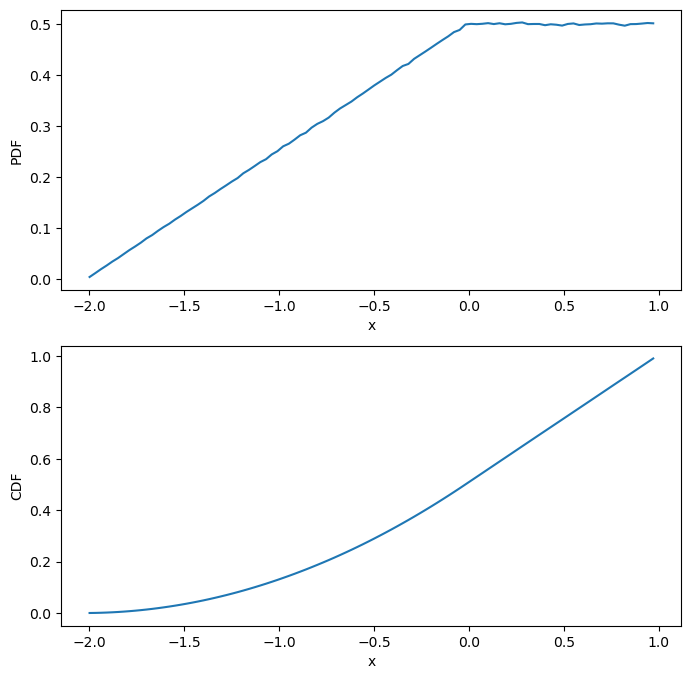
\includegraphics[width=9cm]{./figs/z.png}
    \caption{}
    \label{fig:64ec/2022}
\end{figure}

Simulation steps:
\begin{enumerate}
    \item Create an empty array, $X$, of a desired size $n$.
    \item For every $i$ in the range $[0, n)$, assign $X[i]$ to be $F_X^{-1}(u)$, where $F_X(x)$ is the CDF of X, and $u$ is a random sample belonging to uniform distribution in the range $(0, 1)$.
    \item Write all values stored in $X$ onto a text file, say "vals.txt".
    \item Using python, plot the PDF and CDF of the values stored in "vals.txt".
\end{enumerate}


\end{document}